\cotefile{93}
\scanpage{61}
\mspage{8.}
% archive sheet number: 60

\diagram{\(\begin{array}{@{:~}l@{~:~}c@{~:~}c@{~:~}c@{~:~}c@{~:~}c@{~:~}c}
\hline
 & 1971 & 1972 & 1973 & 1974 & 1975 & 1976\\ \hline
\begin{array}{l}\text{Fonctionnement}\\ \text{(MF) Chap. 36.15}\end{array}
 & 190 & 206 & 223 & 249 & 257 & 275\\ \hline
\begin{array}{l}\text{Equipement (MF)}\\ \text{Chap. 56-10 (50)}\end{array}
 & 87 & 92 & 93 & 93 & 104 & 79\\ \hline
\text{TOTAL} & 277 & 298 & 316 & 342 & 361 & 3\deleted{\unsure{9|5}}\handwritten{5}4\\ \hline
\end{array}\)}

La quasi totalité du crédit de fonctionnement est réparti en tenant compte de critères quantitatifs :

- nombre d'enseignant chercheurs de l'établissement

- nombre de thèses soutenues

- nombre d'association réalisées avec d'autres établissements de recherche

- investissements réalisés au cours des six dernières années au profit des formations de recherche.

- nouvelles actions originales de l'établissement.

Cette répartition est effectuée avant le début de l'année civile. La totalité du budget 1976 est donc actuellement répartie.

Le budget d'équipement est réparti par la D.E.S.U.R. sous la forme de deux grandes masses :

- des constructions spécifiques pour la recherche, et des investissements de matériels de grande importance (ordinateurs, matériels communs à plusieurs établissements) ; ces opérations sont pilotés par la DESUR en accord avec les établissements.

- du matériel "moyen" pour la recherche, ces appareils sont attribués à l'établissement sur sa proposition, après examen et approbation par les experts de la DESUR.

\scanpage{62}
% archive sheet number: 61

\unsure{Celà|Ceci|Cela} \unsure{marche|mène} aussi si \deleted{\unsure{$Z$|$X$}}\inserted{$(\unsure{q_2|q_{0}|\psi_1})$} $Y$ \inserted{cpct} admet \deleted{des} rec.ts arbitrairement fins \inserted{finis} par des $Y_i$ \inserted{fermés ou ouverts} tels que les intersections $Y_{i_1}\cap Y_{i_2}\cap\ \cap Y_{i_{\unsure{r|\nu}}}$ $(\unsure{r|\nu}\geq1)$ de tels $Y_i$ soient $\in\unsure{\mathcal E|\mathscr E}_{\chi!}$ \ldots.

Dans le cas \unsure{du|des} $\chi$, on utilise la suite spectrale d'\uline{homologie}, on est ramené :

\uline{Lemme} Soit $R$ syst. \unsure{loc$^{\mathrm{t}}$|local} de \unsure{$k$-vectoriels|$k$-vectoriel|homotopique} sur $Y\in\mathcal E_\chi$, \unsure{fibres|fibrés} de rang \inserted{fini} $b$. Alors

\[
\chi(Y,R)\overset{\mathrm{d\acute ef}}{=}\sum_p(-1)^p
\underset{\text{le dual est }H^p(Y,\check R)}{\underline{H_p^{\deleted{\unsure{p|\flat}}}(Y,R)}}
\]

existe et

\[
\chi(Y,R)=b\chi(Y)
\]

Cela montre pourvu qu'on fasse l'hyp. \deleted{\unsure{(q$_2$)}} \inserted{que $Y$} est $\sim Y'$ satisfaisant la condition $(\unsure{q_2|q_{0}|\psi_2})$
\begin{center}$=$\end{center}

\deleted{On va se borner}

\textcircled{\unsure{4|h}} Définissons $\mathcal C_{-1}={}$ ens. réduit : l'espace vide

et si $n\geq0$ $\mathcal C_n^{\deleted{\unsure{\mathrm{cpct}}}}={}$ \deleted{catégorie} \inserted{ens.} des espaces cpcts \inserted{$X$} tels que tt pt \inserted{$x\in X$} ait un voisinage $C_x$ tel qu'il existe un espace compact $S\in\mathcal E_{n-1}$ et un homéom. $\mathrm{Cône}(S)\simeq C_x$ transformant le sommet du cône en $x$.

\margin{\uline{NB} $\mathcal E_0$ espaces discrets\\
$\mathcal E_1$ 1-complexes topologiques\\
$\mathcal E_2$ espaces loc. triangulables de dim $\leq2$ [ils sont \unsure{tri-angul.|triangulables} \unsure{ds|dans} le cas cpct]\\
$\mathcal E_3$ espaces loc. triangulables de dim $\leq3$ [\unsure{ils sont tr. triangul.|triangulables} \unsure{ds|dans} le cas cpct]\\
$\mathcal E_4$ esp. loc. \unsure{\textquotedblleft id\textquotedblright} dim $\leq4$ (Moïse) S'ils sont cpcts, il n'est pas clair qu'ils sont triangulables \ldots.}

\[
\mathcal C_\infty=\bigcup\mathcal C_n\qquad\text{(espaces loc. côniques)}
\]

$\mathcal E_\infty={}$ \deleted{\unsure{esp}} des espaces loc. cpcts \inserted{séparés} $X$ tels que $\hat X$ soit loc. cônique i.e. soit $\in C_\infty$.

\[
\text{\uline{Prop}}\qquad \mathcal C_\infty\subset\mathcal E_\chi\cap\mathcal E_{\chi!}
\]

Soit $X\in\mathcal E_\infty$. Si $X$ est cpct, \inserted{donc $X\in C_\infty$} comme $X$ est loc. \unsure{contr. et il|contr. et $L$|contractile}, on sait que $X\in\mathcal E_\chi$, donc $X\in\mathcal E_{\chi!}$. \deleted{\unsure{Cas $X$ quelconque}} \inserted{Sinon} : $X$ loc. cpct $=\hat X-(\omega)$, avec $\hat X\in\mathcal C_\infty$, on a $\hat X\in\mathcal E_\chi$, donc $\hat X-\omega=X\in\mathcal E_{\chi!}$ par (b). Pour prouver $X\in\mathcal E_\chi$, prenons un $C_x\simeq C(S)$, prenons un homothétique $\frac12 C_x=T$, et

\scanpage{63}
\mspage{\unsure{7|1}.}
% archive sheet number: 62

\unsure{-} considération la demande des besoins locaux.

4 - \uline{Comment faire de la recherche dans un établissement d'enseignement supérieur}

4.1. \uline{Les établissements et leurs moyens de base} :

Un établissement d'enseignement supérieur possède du personnel enseignant dont une partie seulement de l'activité est consacrée à l'enseignement ; le reste peut donc être consacré à la recherche. Il est difficile d'avancer une estimation chiffrée de ce partage, qui varie selon les disciplines. Considérons en première approximation que le temps consacré à l'activité de recherche est de 40\% en moyenne du temps de l'enseignant chercheur. Par ailleurs, l'établissement dispose de locaux construits et entretenus à l'aide de crédits inscrits sur des chapitres budgétaires de la D.E.S.U.R. (non inclus dans l'enveloppe recherche\handwritten{)}. Enfin, l'établissement dispose de personnel administratif, technique, ouvrier et de service (A.T.O.S.) dont une part de l'activité est consacrée à la recherche. Il apparait donc d'emblée que chaque établissement possède un potentiel "hors enveloppe-recherche", qu'il doit mobiliser pour le consacrer à la recherche.

Pour chiffrer ce budget, hors enveloppe-recherche, qui est pourtant consacré à la recherche, on pourrait prendre 40\% de la masse salariale des enseignants et admettre, en première approximation, que 30\% du personnel A.T.O.S. effectue un travail de recherche. En admettant en outre qu'une part du budget général du secrétariat d'Etat (chapitre 36-11) contribue à la recherche (ne serait-ce que par le paiement des \unsure{dépenses} de chauffage des bâtiments ...), on arrive en 1975 à une approximation des dépenses pour la recherche de l'ordre de 1~100 à 1~200 millions de francs. Il peut donc être constaté que par le simple fait qu'elle rétribue à plein temps du personnel qui fait de l'enseignement à temps partiel, l'ensemble des établissements de la D.E.S.U.R. apporte au budget "recherche" une somme supérieure au milliard de francs.

4.2. \uline{Les crédits de la D.E.S.U.R. pour constituer ces moyens}

La D.E.S.U.R. dispose de deux chapitres budgétaires,d'un de "fonctionnement", l'autre "d'équipement", qui permettent d'aider cet effort de recherche dans chaque établissement. Le tableau ci-après indique l'évolution de ces budgets (millions de francs courants)

\scanpage{64}
% archive sheet number: 63

soit $X'=\hat X-\mathring T$. qui est cpct. \deleted{\unsure{et $\in C$.|$X\in\mathcal C$.}} On vérifie

\margin{\uline{vérifier}}

\[
\begin{aligned}
\text{a)}\quad & X'\in C_\infty \qquad\text{donc}\quad X'\in \unsure{\mathcal E|\mathscr E}_\chi\\
\text{b)}\quad & X'\sim X=\hat X-\omega \qquad\text{donc}\quad X\in\mathcal E_\chi,
\end{aligned}
\]

\uline{NB} On trouve

\[
\chi(X)=\chi(\hat X-\mathring T)=\chi(\hat X)-\underset{\deleted{\unsure{\Vert\,1}}}{\underline{\chi(T)}}+\chi(\partial T)
\]

et $\chi(T)=1$ car $T$ \unsure{contractible|contr.ible|contractile}, donc

\[
\chi(X)=\chi(\hat X)-1+\chi(\underset{\substack{\Vert\\ S_\omega}}{\underline{\partial T}})=\chi_!(X)+\chi(\partial T)\qquad\text{i.e}
\]

\diagram{\fbox{\begin{tikzcd}[ampersand replacement=\&,column sep=0pt,row sep=1ex]
\chi(X)-\chi_!(X)=\chi( \& S_\omega\arrow[dr,bend right=38] \& )\\
\& \& \substack{\text{exprime la ``structure}\\ \text{locale de $X$ à l'infini''}}
\end{tikzcd}}}

\scanpage{65}
\mspage{6.}
% archive sheet number: 64

3.3. \uline{Les objectifs de recherche spécifiques des établissements d'enseignement supérieur}.

3.3.1. \uline{Mémorisation et diffusion de la connaissance} :

- rassemblement de la connaissance ; conservation de la connaissance ; mise en forme et diffusion de la connaissance. Cette diffusion ne sera pas limitée aux seuls étudiants à plein temps mais étendue vers toute personne intéressée et produite par tous supports(articles, ouvrages, collections, expositions) et toutes prestations (aide technique à l'industrie, études ...). La recherche pédagogique entre dans ce cadre.

3.3.2. \uline{Contribution à l'accroissement de la connaissance}

- en collaborant avec d'autres établissements de recherche, dans le cadre d'associations : l'établissement d'enseignement supérieur apporte une part des moyens, et une part importante du personnel compétent.

- en maintenant un état de "fermentation intellectuelle" permettant de faire naître des nouveaux domaines de recherche, notamment par le contact entre les diverses disciplines\unsure{.|:} Les nouvelles idées de recherche\handwritten{,} initiées par l'établissement\handwritten{,} doivent\deleted{\unsure{,}} ensuite être développées dans le cadre d'associations.

3.3.3. \uline{Formation par la recherche des futurs cadres de la nation.}

- Ceci exige un couplage de l'établissement avec des formations de recherche, où les étudiants en fin d'études pourront aller s'initier à la recherche en préparant une thèse de spécialité. La formation initiale et permanente des enseignants des établissements d'enseignement supérieur entre dans ce cadre. \unsure{-}

3.3.4. \uline{Contribution à l'animation intellectuelle et socio-économique de la région} :

\margin{\unsure{-}}

- Les universités sont en effet les seuls établissements à vocation de recherche qui n'ont pas leur siège à Paris, et dont le programme n'est pas commandé par l'autorité centrale. Elles doivent plus que jamais s'ouvrir aux préoccupations de leur région en prenant en

\scanpage{66}
% archive sheet number: 65

\uline{Th} Sur la cat. $\unsure{\mathcal E|\mathscr E}_\infty$ des espaces loc. cpcts séparés et \deleted{\unsure{cônes|côniq.}} ``loc. côniques partout'' (y compris à l'$\infty$), on peut trouver \deleted{deux} fonctions numériques \inserted{$\chi_!,\chi$} (à valeurs $\in\mathbb Z$) satisfaisant les conditions (où tous les esp. ici écrits sont supposés $\in\mathcal E_\infty$)

\[
\text{\textcircled{a}}\quad\chi_!(X)=\chi(X)\text{ si }X\text{ cpct}
\]

\[
\text{\textcircled{b}}\quad Y\text{ fermé dans }X\ \Longrightarrow\ \chi_!(X)=\chi_!(Y)+\chi_!(X-Y)
\]

\[
\text{\textcircled{c}}\quad X',X''\text{ fermés dans }X\ \unsure{\Rightarrow|=}\ \chi(X)=\chi(X')+\chi(X'')-\chi(X'\cap X'')
\]

\[
\text{\textcircled{d}}\quad\left\{\begin{aligned}
X\sim X' &\Longrightarrow \chi(X)=\chi(X')\\
X\simeq X' &\longrightarrow \chi_!(X)=\chi_!(X')
\end{aligned}\right.
\]

\[
\text{\textcircled{e}}\quad\chi(\mathrm{pt})=1
\]

\[
\begin{aligned}
\text{\textcircled{f}}\quad&\chi_!(X\times Y)=\chi_!(\unsure{x|X})\chi_!(Y)\\
&\chi_{\deleted{\unsure{!|h}}}(X\times Y)=\chi(X)\chi(Y)
\end{aligned}
\]

\textcircled{g}\quad Si $f:X\longrightarrow Y$ fibration loc triviale de fibre $F$,

\[
\left\{\begin{aligned}
\chi_!(X)&=\chi_!(Y)\chi_!(F)\\
\chi(X)&=\chi(Y)\chi(F)
\end{aligned}\right.
\]

tout au moins si $Y$ est un polyèdre relatif (diff. de deux polyèdres, l'un plongé dans l'autre linéairement...)

\margin{j'ignore si c'est vrai sans telle restriction}

Si \deleted{\unsure{$Z$|le}} $X\in\mathcal E_\infty$ de sorte que $\hat X\in\mathcal E_\infty$, on a

\[
\text{\textcircled{h}}\quad\left\{\begin{aligned}
\chi_!(X)&=\chi(\hat X)-1\\
\chi(X)-\chi_!(X)&=\chi(S)\quad\text{où $S$ est la ``frontière à l'infini'' de $X$.}
\end{aligned}\right.
\]

Enfin, \unsure{les restrictions|la restriction} de \deleted{\unsure{$\mathcal E$}} $\chi$ et $\chi_!$ aux polyèdres relatifs sont uniquement déterminées par les propriétés \textcircled{a} à \textcircled{e}, et on a \deleted{\unsure{la}}, si $X$ muni d'une filtration cellulaire

\margin{j'ignore si $\chi$ et $\chi_!$ sont \unsure{caractérisés|caractérisées} par a) à e) sur tout $\mathcal E_\infty$}

\[
\chi_!(X)=\sum(-1)^i\unsure{\hat f_i|f_i}\qquad\text{(formule d'Euler)}
\]

\scanpage{67}
\mspage{5.}
% archive sheet number: 66

3.2. \uline{Les missions d'enseignement et les missions de recherche}

- Les établissements ont-ils des missions de recherche ? C'est là une question à nous poser et à laquelle il importe de répondre en allant au fond du problème.

En effet, la recherche est aujourd'hui une activité fondamentale pour la nation ; des milliers de travailleurs y consacrent la totalité de leur activité, dans le cadre du"plan recherche". On pourrait se demander s'il est nécessaire que les enseignants des établissements d'enseignement supérieur y consacrent aussi une part de leur activité... Il n'est pas évident que l'on puisse faire du bon travail à temps partiel à l'époque d'intense compétition internationale qu'est la notre. Vaudrait-il mieux peut être, développer un peu plus l'effort de recherche et découpler totalement l'enseignement et la recherche, à l'époque où l'enseignement supérieur ne peut plus revendiquer un monopole dans cette activité ?...

On ne peut ignorer que la question se pose en ces termes à de nombreuses personnes. \unsure{-}

- Face à cette intérrogation, la D.E.S.U.R. a donc défini très clairement des objectifs spécifiques pour la recherche menée dans les établissements qui doivent donc s'appeler établissements d'enseignement supérieur et de recherche. La base du raisonnement est la suivante :

\noindent\fbox{\parbox{0.95\linewidth}{Une centaine d'établissements autonomes, dont la plupart ont leur siège social en province, exercent en priorité des missions d'enseignement. Toutefois, leur personnel enseignant, formé par la recherche, est disponible à temps partiel pour contribuer à l'effort national de recherche. Du fait même qu'il est enseignant, il peut remplir des missions de recherche spécifiques, indispensabl\unsure{\={e}|e}s à l'effort national de recherche. Cet effort de recherche permet sa formation permanente et la formation de jeunes chercheurs\handwritten{,} contribu\deleted{\unsure{e|a}}ant ainsi à maintenir l'établissement en pleine activité créatrice.}}

Il faut définir, à partir de ces données, des objectifs de recherche pour les établissements d'enseignement su\deleted{\unsure{ép|pé}}périeur. Ceux-ci pourront tout en contribuant à l'effort national de recherche, se développer eux-mêmes pour le plus grand bien de leur mission fondamentale d'enseignement.

\scanpage{68}
% archive sheet number: 67

\unsure{orientations|orientation}

\unsure{plongements|plongement}

$H_i,\chi$

\[
\left\{\begin{aligned}
&\text{rev. et }\pi_1\\
&\text{rel. entre }\pi_1\text{ et th. de Galois}\\
&\text{rev. et fonctions de var. }\text{\unsure{complexe|complexes}}
\end{aligned}\right.
\]

Conj. de Weil

\scanpage{69}
% archive sheet number: 68

\figure{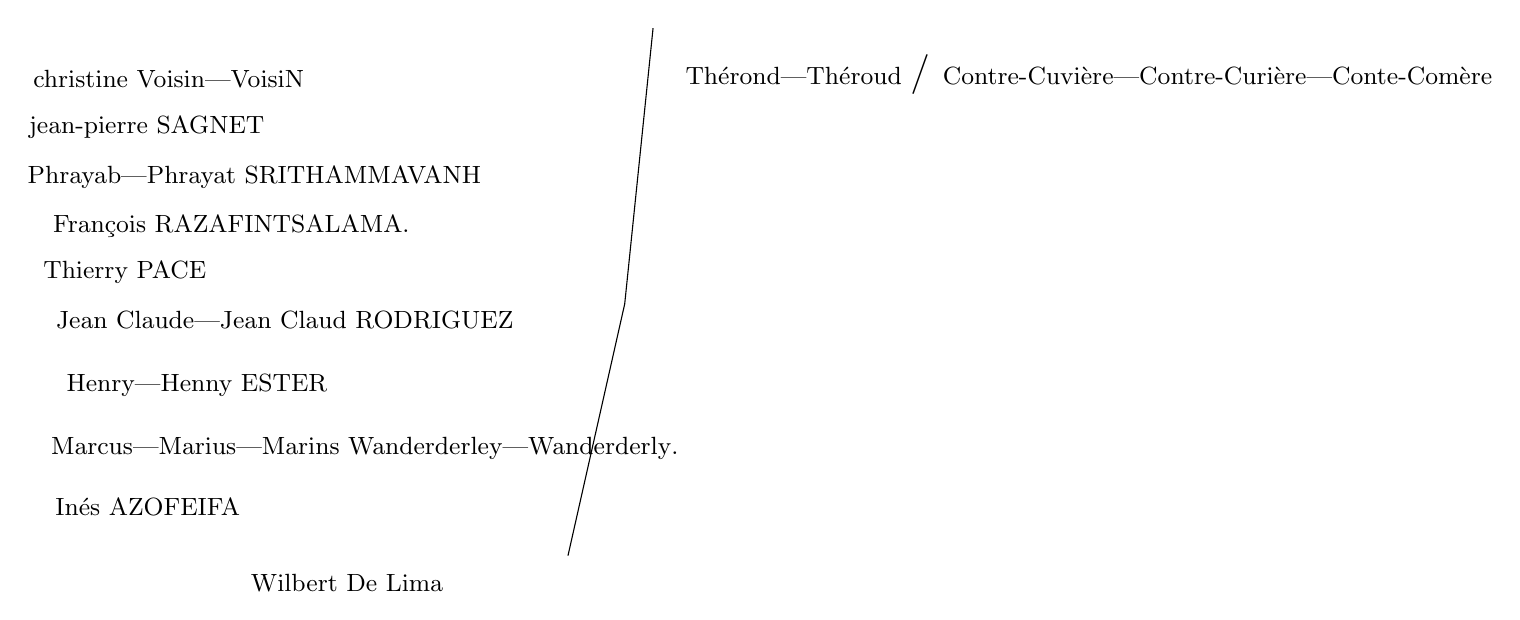
\begin{tikzpicture}[x=0.009cm,y=-0.009cm,every node/.style={anchor=base west,inner sep=0pt,font=\small}]
\draw (890,1)--(850,390)--(770,745);

\node at (15,84) {christine \unsure{Voisin|VoisiN}};

\node at (935,80) {\uline{\unsure{Thérond|Théroud}} \Large/ \small\uline{\unsure{Contre-Cuvière|Contre-Curière|Conte-Comère}}};

\node at (9,150) {jean-pierre SAGNET};

\node at (7,220) {\unsure{Phrayab|Phrayat} SRITHAMMAVANH};

\node at (43,289) {François RAZAFINTSALAMA.};

\node at (29,354) {Thierry PACE};

\node at (47,425) {\unsure{Jean Claude|Jean Claud} RODRIGUEZ};

\node at (62,513) {\unsure{Henry|Henny} ESTER};

\node at (40,603) {\unsure{Marcus|Marius|Marins} \unsure{Wanderderley|Wanderderly}.};

\node at (46,689) {Inés AZOFEIFA};

\node at (322,796) {Wilbert De Lima};
\end{tikzpicture}}

\scanpage{70}
% archive sheet number: 69
% The thick backslash and the pale mirror writing show through from scan 69.

7 rue \unsure{Daru|Dare}\\

\unsure{Basane|Bazane|Barane}

\scanpage{72}
% archive sheet number: 71

\uline{Th} \textcircled{I} Soit $X$ une courbe analytique régulière, $\deleted{\unsure{\mathcal P_X|\mathcal E_X}}\inserted{\unsure{\mathcal E|\mathscr E}_X}\ (\unsure{\mathcal P|\mathscr P}_X)$ le faisceau des applications étales d'ouverts de $X$ dans $\mathbb E^1(\mathbb C)$ $(\mathbb P^1(\mathbb C))$. Il existe un morphisme

\[
G:\mathcal E_X\times\mathcal E_X\longrightarrow\underline\omega_{X/\mathbb C}^{\otimes2}
\qquad(\underline\omega_{X/\mathbb C}=\underline\Omega^1_{X/\mathbb C})
\]

ayant les propriétés suivantes

a) $G$ est un op. différentiel (pas néc linéaire), i.e. en termes d'une uniformisante locale $t$ \inserted{(déf. sur un ouvert $U$)} on a

\[
G(f,g)=R(f,f',\ldots,f^{(n)},g,g',\ldots,g^{(n)})\,dt^2
\]

$R$ est une fonction rationnelle en $\unsure{2n|2m}$ variables, à coefficients dans $\Gamma(\unsure{U|X},\mathcal O_U)$. De plus, \deleted{\unsure{le dénominateur|le dénominateur n'est}} \inserted{si $R=P/Q$, $P$ et $Q$ polynômes,} $Q$ non identiquemt nul, \deleted{si on substitue} ce qui implique \deleted{\unsure{est tel qu'il n'a pas de pôles zéros}} que $Q(f,\unsure{g'|f'},\ldots,f^{(n)};g,g',\ldots,g^{(n)})$ n'est pas identiquemt nul, \deleted{\unsure{quel que soit le choix de $f$}} \inserted{\unsure{$f$ et $g$}} on suppose que $Q$ ne s'annule identiquemt pour aucuns $f$ et $g$ avec $f$ et $g$ non loc. constantes ni l'une ni l'autre, et que $P(f,\ldots,g,\ldots)/Q(f,\ldots,g,\ldots)$ n'a \deleted{pas} de pôles qu'aux pts où $f',g'$ ont des zéros.

[On doit pouvoir montrer que, si on prend $P,Q$ premiers entre eux, on \deleted{aura} \inserted{peut prendre} $Q={f'}^{p}{g'}^{q}$, donc

\[
G(f,g)=\frac{1}{{f'}^{p}{g'}^{q}}\,P(f,f',\ldots,f^{(n)};g,g',\ldots,g^{(n)})\quad]
\]

\[
\text{b)}\quad G(f,g)+G(g,h)=G(f,h)
\]

\[
\begin{aligned}
\text{c)}\quad G(f,ag)&=G(f,g)\deleted{\unsure{{}+G(g,\tfrac1g)|{}=G(f,\tfrac1g)}}&
 a\in\mathbb C^*\quad\deleted{\text{si }a\in\mathbb C^*,b\in\mathbb C}\\
G(f,g+b)&=G(f,g)& b\in\mathbb C\quad\deleted{\unsure{\text{et }g|\text{et}}}\\
G(f,1/g)&=G(f,g)&\text{si $g$ sans zéros}
\end{aligned}
\]

d) \deleted{\unsure{Pour $f$ fixé,|Deux $f$ fixés,}} Si $G(f,g)=0$ et $f,g$ coïncident à l'ordre 2 en un point $x\in X$ (\unsure{i.e.} $f,g\in\Gamma(U,\underline{\mathcal O}_U)$) alors $f=g$ si $U$ connexe.

% margin note written sideways
\margin{e) Si $f\in\Gamma(U,\mathcal E_U)$, le morphisme $g\longmapsto G(f,g)$ de $\mathcal E_U$ dans $\underline\omega_U^{\otimes2}$ est un épi}

% margin note written sideways
\margin{\uline{NB} c) implique que $G$ \unsure{soit défini|se définit|se factorise en} sur $\mathcal P_X\times\mathcal P_X\longrightarrow\underline\omega_X^{\otimes2}$, \deleted{\unsure{et se factorise en}} \inserted{\unsure{et signifie qu'il est}} $\,{}_H\backslash\mathcal P_X\times {}_H\backslash\mathcal P_X\longrightarrow\underline\omega_X^{\otimes2}$, où $H=\mathrm{GP}(1,\mathbb C)$. b) donne la relation analogue pour $\,{}_H\backslash\mathcal P_X$, d'où torseur $\mathcal T_X$ et $\,{}_H\backslash\mathcal P_X\xrightarrow{c}\mathcal T$ avec $G(f,g)\unsure{\equiv|=}c(f)-c(g)$; Alors d) signifie que $\unsure{{}_H\backslash\mathcal P_X|\mathcal P_X}\xrightarrow{c}\mathcal T_X$ est mono, et e) que c'est épi}

Deux tels morphismes $G'$ et $G$ sont liés par

\[
G'=\varphi G,\qquad\text{avec }\varphi\in\Gamma(X,\underline{\mathcal O}_X^*)
\]

\textcircled{II} Si, au lieu de prendre $X$ fixe, on prend $X$ variable, avec morphismes étales entre des $X$, on a $=$ résultat, et l'indétermination sera

% margin note written sideways
\margin{Ici, au lieu des conditions d), e) il suffit de supposer d) \deleted{\unsure{que $G$ est fidèle}}}

\[
G'=c\,G\qquad c\in\mathbb C^*
\]

\unsure{TSVP|TSVo}

\scanpage{73}
% archive sheet number: 72

[Ici, on montre que \inserted{la condition a) implique que} pour tt $X$ fixé, l'expression de a), $G(f,g)=R(f,f',\ldots,f^{(n)};g,\unsure{g|g'},\ldots,g^{(n)})$ doit avoir des coefficients $\in\mathbb C$, indépendants de $X$, donc

\[
R\in\mathbb C(F_0,F_1,\ldots,F_n;G_0,\ldots,G_n)
\]

et en fait, $R(\quad)=\underbrace{P(F_0,\ldots;G_0,\ldots)}_{\in\mathbb C[F_0,\ldots,G_0\ldots]}/F_1^p G_1^q$ \hfill ]

On peut prendre

\[
G(f,g)=\biggl(\left[-2\,\frac{g'''}{g'}+3\left(\frac{g''}{g'}\right)^2\right]-
 \left[-2\,\frac{f'''}{f'}+3\left(\frac{f''}{f'}\right)^2\right]dt^2
\]

De plus, on trouve un torseur canonique $\mathcal T_X$ \deleted{\unsure{sous|sur}} $\underline\omega^{\otimes2}_{X/\mathbb C}$, \unsure{dépend|dépent|dépendant} fonct\unsure{ionellt|ionellement|oriellt|oriellement} de $X$ (pour morphismes étales), et

\[
\deleted{\unsure{c_0|G_0}}\ c^X:\mathcal P_X\longrightarrow\mathcal T_X
\]

tel que

\[
\left\{\begin{aligned}
G(f,g)&=c^X(g)-c^X(f)\\
c^X&\text{ se factorise en } \!{}_H\backslash\mathcal P_X\longrightarrow\mathcal T_X\\
&\text{Ce dernier morphisme est un iso}
\end{aligned}\right.
\]

\uline{III}) On prend maintenant $X$ \inserted{schéma} variable lisse (ou seulement diff. lisse à l'ordre 3) sur des schémas variables, et on cherche pour tt tel $X$

\[
\unsure{\mathcal E_X|\mathscr E_X}\times\mathcal E_X\xrightarrow{G}\omega^2_{X/S}
\]

de façon compatible avec chgt de base $S'\to S$, avec morphismes étales

\diagram{\begin{tikzcd}[ampersand replacement=\&,column sep=small,row sep=small]
X'\arrow[rr]\arrow[dr,dash] \& \& X\arrow[dl,dash]\\
\& S \&
\end{tikzcd}}

, et satisfaisant les conditions qui correspondent à \inserted{$\Rightarrow$ b), c),} (\uline{plus} les condition d) \deleted{\unsure{e)}} \inserted{si \deleted{\unsure{on|si}} $S$ corps de car. 0, et e) dans} \deleted{\unsure{b), c) du cas précédent de l'} analytique complexe}).

% slanted
\margin{la forme suivante : $G(f,g)$ n'est \unsure{identiq$^{\mathrm{mt}}$|ident.} nul en aucune carct. $p>0$}

Mais quand on parle d'``op. différentiel'', il faut maintenant remplacer un polynôme $R$ en $f,f',f'',\ldots,g,g',g'',g'''$ par un polynôme en $f,f'=D_t^{(1)}f,D_t^{(2)}(f)\ldots D_t^{(n)}f,\ g,g'=D_t^{(1)}g,D_t^{(2)}g,\ldots D_t^{(n)}g$. \deleted{On voit comme} A priori, les coeff. sont dans $\Gamma(U,\underline{\mathcal O}_U)$. (si $t$, \deleted{\unsure{est|de}} l'uniformisante, est définie sur $U$) mais si on \deleted{\unsure{f|p}} veut faire varier $X$, on voit que les coefficients doivent être \uline{dans $\mathbb Z$} (ou dans

$\Gamma(S_0,\underline{\mathcal O}_{S_0})$ si on a fixé un schéma de base commun $S_0$ pour les $S,X\ldots$). On trouve encore l'existence d'un tel, et l'unicité à un facteur $\varepsilon\in\mathbb Z^*$ près, i.e. $\varepsilon=\pm1$ : \uline{unicité au signe près} ! Ici, on ne peut prendre l'expression $G'(f,g)$ précédente, car elle est identiq$^{\mathrm{mt}}$ nulle en car. 2 et 3 ! Il faut prendre $\frac1{12}G(f,g)$, savoir

\[
G_0(f,g)=\left[\left(-\frac{D_t^{(3)}g}{D_t^{(1)}g}+\left(\frac{D_t^{(2)}g}{D_t^{(1)}g}\right)^2\right)
-\left(-\frac{D_t^{(3)}f}{D_t^{(1)}f}+\left(\frac{D_t^{(2)}f}{D_t^{(1)}f}\right)^2\right)\right]dt^2
\]

Pour caractériser ce choix (parmi les deux possibles au signe près) on va calculer p.ex

\[
G_0(t,t^2)=\deleted{\unsure{\frac1{2t}dt^2|\frac1{2}dt^2|\frac1{2t}}}\ \frac1{2t}dt^2\qquad
\text{(au lieu de }-\tfrac1{2t}\,dt^2\text{)}
\]

[Il ne faut pas s'effrayer du dénominateur, pour le cas où 2 n'est pas inv. sur $X$ : alors $t^2$ n'est jamais une uniformisante !] ou bien soit quelque chose qui ait un sens aussi en car 2

\[
G_0(t,t^3)=\underbrace{\left(-\frac1{3t^2}+\left(\frac{3t}{3t^2}\right)^2\right)}_{\frac1{t^2}(-\frac13+1)}dt^2
=\deleted{\unsure{\frac1{3t^2}|\frac1{3t}}}\ \frac23\,\frac1{t^2}dt^2
\]

[mais c'est inutile, car en car 2 les \deleted{\unsure{définit$^{\mathrm{ns}}$|définitions|différents}} \inserted{deux choix} possibles sur $\mathbb Z$ coïncident !].

\uline{Rem.} 1) On peut se demander quel est le rôle joué dans cet énoncé par les biformes, et s'il n'y aurait pas moyen d'éliminer ce rôle. On est alors conduit, dans I), à se donner un faisceau analytique coh. $\mathcal F$ sur $X$, et à supposer $G'\deleted{\unsure{(f,g)|f,g}}:\mathcal E_X\times\mathcal E_X\longrightarrow\mathcal F$. On trouve alors qu'un tel $G'$ s'écrit de façon unique (où $G$ est comme dans l'énoncé initial, p.ex. celui de II) comme $G'=uG$, où $u:\underline\omega_X^{\otimes2}\longrightarrow\mathcal F$, et $u$ est même un \uline{iso} ! Donc $\underline\omega_X^{\otimes2}$ joue ici un rôle \uline{universel}. Dans II) on pourrait se donner un $\mathcal F_X$ dépd$^{\mathrm{t}}$

\scanpage{74}
% archive sheet number: 73

\unsure{fonctoriellt|fonctoriellement} de $X$, mais on trouverait encore un iso fonctoriel en $X$, $\mathcal F_X\simeq\underline\omega^{\otimes2}_{X/\mathbb C}$. \deleted{De} \unsure{$=$|''} dans (\unsure{III|II}). Ainsi les 2-formes sont essentielles.

2) \deleted{G} Le torseur $\mathcal T$ dont il est question dans II (et en marge de I) dépend du choix de $G$ (et de $\mathcal F$, si on veut -- c'est alors un torseur sous $\mathcal F$) mais les \inserted{torseurs associés aux} différents choix sont can. (semi)-isomorphes, de façon précise

\[
\mathcal T^G\xrightarrow{\sim}\mathcal T^{\varphi G}
\]

\unsure{corresp. avec|comp. avec|au-dessus de}

\[
\underline\omega_X^{\otimes2}\xrightarrow{\varphi.\mathrm{id}}\underline\omega_X^{\otimes2}
\]

i.e. $\mathcal T^{\varphi G}$ est ``multiplié'' de $\unsure{\mathcal E^G|\mathcal T^G}$ par $\varphi$. Ainsi, le choix ``le plus fin'' de $\mathcal T$ est $\mathcal T^{G_0}$ (où $G_0$ est défini en (III)), alors le $\mathcal T^G$ correspondant \deleted{au choix} \inserted{$G$} de (\unsure{II|III}) est un multiple 12 ième de $\mathcal T^{G_0}$.

3) On \unsure{peut|pourrait} se \deleted{demander} \inserted{poser} la question de caractériser $G_0(f,g)$ \uline{en une caractéristique donnée} $p>0$. On peut prendre les conditions a) \inserted{\unsure{reprises|reçues} comme plus haut} b) c), plus d') que $G_0(f,g)$ n'est pas id. nul -- \uline{cela caractérise} $G_0(f,g)$ à multiplication près par une constante $c\in\mathbb F_p^*$. \unsure{M̄|M.} précis$^{\mathrm{t}}$, si on se fixe un schéma de base absolu \uline{intègre} $S_0$ (pour les $S$ et les $X$), l'indétermination est dans $\Gamma(S,\mathcal O_S^*)$. Si $S$ n'est pas intègre, il faut supposer que, sur chaque $k(s)$, l'op. induit (pour des $X$ lisses \deleted{\unsure{sur le|sur une}} \inserted{de dim$^{\mathrm{ion}}$} rel. 1 sur $k(s)$, )

% slanted
\margin{\uline{faux} ?! \unsure{car un|par un|si} \unsure{$D_W$|sur $W$} ou \unsure{déjà|déf.|diff.} \unsure{$G$} d'ordre $\leq3$)}

% margin note written sideways
\margin{\unsure{$d$|$G$|d')} n'est pas identiquement nul.}

\scanpage{75}
% archive sheet number: 74

Les développements précédents étaient centrés sur le groupe $H=\unsure{\mathrm{Gp}(1,\mathbb C)|\mathrm{GP}(1,\mathbb C)}$ opérant sur $\mathbb P^1(\mathbb C)$ (ou $\mathrm{Gp}(1)_{\mathbb Z}$ sur $\mathbb P^1_{\mathbb Z}\ldots$), et les \unsure{invariants|invariant} différentiels, sous l'action de ce groupe, des fonctions analytiques complexes (\uline{NB} marcherait aussi dans l'analytique réel, ou les $C^\infty$, voire $C^3$). On va passer rapidement en revue les développements analogues pour d'autres groupes

a) \uline{Groupe des translations} $\mathbb G_a$ \uline{opérant sur} $\mathbb E^1$

On a l'opération (dans l'analytique complexe p.ex)

\[
d:\underline{\mathcal O}_X\longrightarrow\underline\Omega^1_{X/\mathbb C}=\underline\omega_X
\]

% slanted
\margin{\uline{Ici} $\underline{\mathcal O}_X$ mauvais pt de vue, prendre $\unsure{\mathcal E_X|\mathscr E_X}$ plutôt !}

qui est \inserted{épi ($X$ lisse dim 1) et} nul \deleted{exactement} sur les fonctions loc. constantes, donc posant

\[
A(f,g)=dg-df,\qquad A:\underline{\mathcal O}_X\times\underline{\mathcal O}_X\longrightarrow\underline\omega_X
\]

on trouve l'analogue de a) b) dessus, plus

\[
 A(f,g+c)=A(f,g)\qquad c\in\mathbb C
\]

plus

\[
 A(f,g)=A(f,h),\quad g(x)=h(x)\implies \underset{\text{au vois. de }x}{g=h}
\]

et

\[
g\mapsto A(f,g)\qquad \underline{\mathcal O}_X\longrightarrow\underline\omega_X\quad \text{épi}
\]

.(Cas $X$ lisse de dim 1 pr. \unsure{st. mt|smt|définition}) --

Ici est pas la peine d'introduire de torseur, \inserted{(si on veut, il est trivial)} ni $=$ $A(f,g)$, car l'expression $dg$ contient \unsure{toutes les|tous les} qui en sortent
